\documentclass[conference]{IEEEtran}
\hyphenation{op-tical net-works semi-conduc-tor IEEEtran}
\usepackage[bottom=2cm,top=3cm,left=3cm,right=2cm]{geometry}
\usepackage{url}
\usepackage{amsmath}
\usepackage{amsfonts}
\usepackage{graphicx}
\usepackage[colorinlistoftodos]{todonotes}
\usepackage{algorithm}
\usepackage{algpseudocode}

\makeatletter
\def\ps@pprintTitle{%
	\let\@oddhead\@empty
	\let\@evenhead\@empty
	\def\@oddfoot{\reset@font\hfil\thepage\hfil}
	\let\@evenfoot\@oddfoot
}
\makeatother

\usepackage{babelbib}

\usepackage[brazilian]{babel} % Traduz alguns termos para o português
\usepackage[utf8]{inputenc} % Reconhece acentuação
\usepackage{setspace}
\usepackage{graphicx}


\begin{document}

% paper title
\title{Teoria da Decisão\\Projeto Prático Assistido Por Otimização Multiobjetivo e Métodos de Auxílio à Tomada de Decisão}


% author names and affiliations
% use a multiple column layout for up to three different
% affiliations
\author{\IEEEauthorblockN{Rafael Carneiro de Castro}
\IEEEauthorblockA{\\Eng. de Sistemas - UFMG\\
Matrícula: 2013030210\\
Email: rafaelcarneiroget@hotmail.com}
\and
\IEEEauthorblockN{Vinícius Felicíssimo Campos}
\IEEEauthorblockA{\\Eng. de Controle e Automação - UFMG\\
	Matrícula: 2015035235\\
	Email: viniciusfc95@gmail.com}
\and
\IEEEauthorblockN{Davi Pinheiro Viana}
\IEEEauthorblockA{\\Eng. de Sistemas - UFMG\\
	Matrícula: 2013029912\\
	Email: daviviana22@gmail.com}
}

\maketitle

\begin{abstract}
Abordagem de forma conjunta de grande parte dos conceitos vistos na disciplina "ELE088 - Teoria da Decisão", através de um problema relacionado ao gerenciamento ótimo da política de manutenção de um conjunto de equipamentos de uma empresa. O problema foi resolvido através de modelagem e implementação multiobjetivo e, para verificar a resolução do problema, é apresentado um indicador de qualidade. Além disso, foram utilizados alguns métodos de auxílio à tomada de decisão.
\end{abstract}

\IEEEpeerreviewmaketitle

\section{Introdução}
O presente trabalho tem o objetivo de resolver um problema de otimização multiobjetivo e, utilizando técnicas escalares de decisão assistida estudadas em sala de aula, encontrar a melhor solução para este problema, colocando em prática grande parte dos conceitos da matéria.

O problema a ser resolvido é o seguinte: \emph{Deseja-se determinar a política de manutenção ótima para cada um dos 500 equipamentos de	uma empresa, considerando-se a minimização do custo de manutenção e a minimização do custo de falha esperado.}

No problema, o custo de manutenção total é a soma dos custos dos planos de manutenção adotados para todos os equipamentos. Sendo que, o valor do custo de cada plano de manutenção é dado. O custo esperado de falha de cada equipamento $i$, sob o plano de manutenção $j$, é o produto da probabilidade de falha ($p_{i,j}$) e o custo de falha do equipamento (este último é dado). O
custo esperado de falha total é a soma dos custos esperados de falha de todos os equipamentos.

Deve ser feita a formulação e resolução do problema multiobjetivo e o resultado encontrado deve ser avaliado baseado no indicador de qualidade hipervolume (s-metric). Esse indicador é utilizado para mensurar as propriedades de convergência e diversidade da fronteira Pareto "aproximada" obtida.

Além disso, deve ser aplicada também a utilização de técnicas de análise de decisão ELECTRE II, PROMETHEE II \emph{fuzzy} e AHP para decidir qual a melhor solução dentre as encontradas para o problema.

\section{Desenvolvimento}
\subsection{Formulação do Problema:}
A formulação do problema foi dividida em duas partes, como é discutido a seguir:

\subsubsection{Minimização do custo de manutenção total} Em primeiro
momento, é preciso construir uma função objetivo e suas eventuais restrições para minimização do custo de manutenção total. Considerando $C_i(x_i)$ como o custo de manutenção do equipamento $i$ em função do plano de manutenção $x_i$, têm-se a seguinte formulação:

\begin{equation}
\mathrm{min}\ \sum_{i=1,}^{n} C_i (x_i) 
\label{sum_cm}
\end{equation}

sujeito a:
\begin{equation}
x_i \in \mathcal{X}\ \forall i\ \in 1, ..., n
\label{rest1_cm}
\end{equation}
\begin{equation}
C_i \in \mathcal{C}\ \forall i\ \in 1, ..., n
\label{rest2_cm}
\end{equation}
Em que $n$ é o número de equipamentos que, no caso do problema a ser resolvido, é igual a 500. A equação \ref{sum_cm} representa o custo de manutenção total que é o somatório dos custos de manutenção de cada equipamento $i$. A restrição \ref{rest1_cm} indica que cada equipamento $i$ pode ter um plano de manutenção $x_i$ que esteja dentro do conjunto $\mathcal{X}$ de planos pré-definidos, no caso do problema, $\mathcal{X} = \{1,2,3\}$. A restrição \ref{rest2_cm} indica que o custo de manutenção de cada equipamento também deve estar dentro de um conjunto pré-definido $\mathcal{C}$ que depende do plano de manutenção.

\subsubsection{Minimização do custo esperado de falha total}

\subsection{Algoritmo de Solução:}
Nesta seção serão discutidos e exibidos os algoritmos para solução do problema multiobjetivo.

Olhando para a equação \ref{sum_biobj} é possível perceber que, minimizando o custo de cada equipamento, minimiza-se também o somatório dos custos. Assim, para resolução do problema biobjetivo foi utilizada uma estratégia gulosa. Nela, para cada equipamento, é feito um teste com cada um dos planos de manutenção e é escolhido aquele que gera menor custo. Têm-se então, um algoritmo cuja complexidade é O($n\cdot m$) em que $n$ é o número de equipamentos e $m$ é o número de planos de manutenção. No caso do problema a ser resolvido no trabalho, para cada par de pesos escolhido (encontrar solução da fronteira Pareto), são feitas 1500 avaliações da função objetivo. Segue, abaixo, um pseudocódigo do funcionamento do algoritmo:

\begin{algorithm}
	\caption{Estratégia gulosa}
	\begin{algorithmic}[1]
		\For{$i = 1$ to ${n}$}
			\State $cBest = w_1 \cdot c_m(\mathcal{X}_1) + w_2 \cdot c_f(\mathcal{X}_1)$
			\State $x_i = \mathcal{X}_1$
			\For{$j = 2$ to ${m}$}
					\If {$(w_1 \cdot c_m(\mathcal{X}_j) + w_2 \cdot c_f(\mathcal{X}_j)) < cBest$}
					\State $cBest = w_1 \cdot c_m(\mathcal{X}_j) + w_2 \cdot c_f(\mathcal{X}_j)$
					\State $x_i = \mathcal{X}_j$
					\EndIf
			\EndFor
		\EndFor
		
	\end{algorithmic}
\end{algorithm}

Essa estratégia foi escolhida por ser simples de implementar e por retornar uma solução exata para o problema. Além disso, é uma solução relativamente barata computacionalmente e que retorna o resultado rapidamente.

O algoritmo que utiliza a estratégia gulosa para resolver a função objetivo pode ser encontrado no arquivo \texttt{Guloso.m} e o algoritmo que implementa a \emph{Soma Ponderada} variando os pesos da função objetivo pode ser encontrado no arquivo \texttt{SomaPonderada.m}, ambos no mesmo diretório deste relatório.

\subsection{Resultados:}
Os algoritmos foram implementados e, na \emph{Soma Ponderada}, foram encontradas 1000 soluções na fronteira pareto, variando os pesos da seguinte forma: $w_1$ varia de 0 a 1 com o passo igual a $0,001$ e $w_2 = 1 - w_1$. Foi encontrada a seguinte fronteira Pareto:

\begin{figure}[h]
	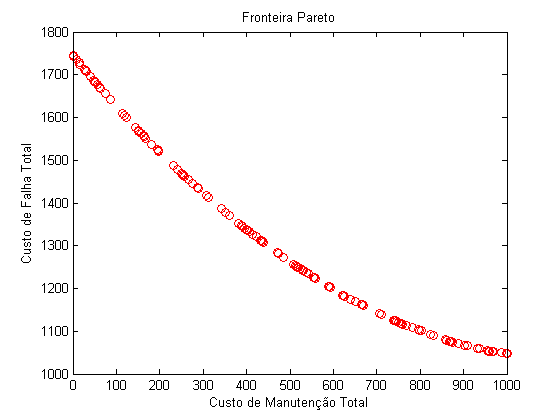
\includegraphics[width=8cm]{img/pareto.png}
	\caption{Froteira Pareto encontrada}
	\label{fig:pareto}
\end{figure}


\subsection{Análise baseada no Hipervolume:}
Com o objetivo de avaliar a Fronteira Pareto encontrada, foi utilizada a análise baseada no indicador de qualidade hipervolume (s-metric). Segundo a especificação do trabalho, um bom valor para o HVI (Valor do Hipervolume) deveria estar acima de $0,6$. Utilizando o algoritmo fornecido pelo professor, foi feita uma execução com a Fronteira Pareto encontrada e o valor de HVI foi igual a $0,621246$. Conclui-se, então, que a fronteira encontrada convergiu para uma quantidade boa de soluções e que pode ser utilizada na análise de tomada de decisão da melhor solução.

\section{Tomada de Decisão Assistida:}
\subsection{Electre II}
O método {\it Elimination and Choice Expressing the Reality} proposto por B. Roy em 1968, também conhecido por ELECTRE I, permite que se determine uma pré-ordem total de ações dado um conjunto de critérios. Este resultado é obtido após a execução de um número significante de passos, a fim de se determinar as relações de sobreclassificação entre duas ações. Seguindo os mesmos princípios, o método ELECTRE II se diferencia do I ao definir duas relações de classificação, a forte e a fraca, e  foi utilizado neste trabalho como um dos métodos de auxílio de tomada de decisão.

As ações a serem ordenadas são os planos de manutenção que compõem a fronteira Pareto obtida previamente. Os critérios são o menor custo de manutenção ($c_1$) e o menor custo de falha esperado ($c_2$). A partir destas definições, os seguintes passos foram executados:

\begin{enumerate}
	\setlength\itemsep{1em}
	\item {\it Ajustar a escala dos valores:} Os custos foram reescalados de forma que os máximos após o processo fossem iguais ao máximo valor inicial dentre ambos os critérios, e os mínimos, iguais à zero. Além disso, como deseja-se obter os menores valores possíveis, a escala foi invertida subtraíndo cada valor do máximo. 
	
	\item {\it Definir os pesos $w_j$ para cada um dos J = {1, ..., $n_c$} critérios:} Dois conjuntos de pesos foram considerados, $w_1 = 0.7$ e $w_2 = 0.3$ e vice-versa. Estes valores foram definidos de forma a representar dois tipos de decisor, aquele que prefere gastar menos agora com manutenção do que com as falhas prováveis no futuro e o seu oposto. Já aquele que não tem preferência neste sentido ($w_1 = w_2 = 0.5$) não foi considerado pois o conjunto de planos apresenta a característica de que quanto melhor um critério, pior o outro, de forma a apresentar indiferença entre as soluções.
	
	\item {\it Estebelecer comparações par a par gerando os seguintes índices:}
	
	\begin{center}
		$J^+(a_i, a_k) =  \{j \in J | c_j(a_i) > c_j(a_k)\}$\\
		$J^=(a_i, a_k) =  \{j \in J | c_j(a_i) = c_j(a_k)\}$\\
		$J^-(a_i, a_k) =  \{j \in J | c_j(a_i) < c_j(a_k)\}$\\
	\end{center}
	
	\item {\it Converter as relações entre as ações em valores numéricos:}
	
	\begin{center}
		$P^+(a_i, a_k) = \sum_{j}{} w_j, j \in J^+(a_i, a_k)$\\
		$P^=(a_i, a_k) = \sum_{j}{} w_j, j \in J^=(a_i, a_k)$\\
		$P^-(a_i, a_k) = \sum_{j}{} w_j, j \in J^-(a_i, a_k)$\\
	\end{center}
	
	\item {\it Calcular os índices de concordância:}
	
	\begin{center}
		$C_{ik} = \frac{P^+(a_i, a_k) + P^=(a_i, a_k)}{\sum_{j \in J}w_j}$\\
	\end{center}
	
	\item {\it Estabeler as relações de sobreclassificação forte ($S_s$):}
		Um plano fortemente sobreclassifica outro no critério j se
		\begin{center}
			$C_{ik} \ge c^+$\\
			e $ c_j(a_k) - c_j(a_i) \le D $\\
			e $ \frac{P^+_{ik}}{P^-_{ik}} \ge 1$\\
		\end{center}
		
		As constantes utilizadas neste passo foram determinadas analisando-se os valores de $P_{ik}$. São elas
		
		\begin{center}
			$c^+= 0.65$\\
    		$D = 0.75 * max(c_1, c_2)$\\
		\end{center}
		
	\item {\it Estabeler as relações de sobreclassificação fraca ($S_w$):}
		Um plano fracamente sobreclassifica outro no critério j se
		\begin{center}
			$C_{ik} \le c^-$\\
			e $ c_j(a_k) - c_j(a_i) \le D $\\
			e $ \frac{P^+_{ik}}{P^-_{ik}} \ge 1$\\
		\end{center}
		
		Sendo
		
		\begin{center}
			$c^-= 0.35$\\
		\end{center}
		
	\item {\it Obter a ordem das soluções:} O processo de classificação original do ELECTRE II propõe duas etapas, a direta e a reversa. Entretanto, devido aos resultados obtidos nos itens anteriores, em que uma ação da matriz $S_s$ sobreclassifica fortemente as ações seguintes e em que $S_w$ está vazia, a ordenação foi obtida de forma direta. Isto é, a ordem foi estabelecida de acordo com o número de vezes que uma ação sobreclassifica fortemente as demais.
\end{enumerate}

Após a execução destes passos, o ELECTRE II apresentou os seguintes resultados:
\begin{itemize}
	\item {\it Para $w_1 = 0.7$ e $w_2 = 0.3$:} Designar planos de manutenção detalhada para as máquinas 36, 204, 318 e 358, enquanto as demais podem ficar sem plano. O custo de manutenção desta alternativa é $8$ e o custo de falha esperado é $1735.2$.
	\item {\it Para $w_1 = 0.3$ e $w_2 = 0.7$:} Designar planos de manutenção detalhada para todas as máquinas. O custo de manutenção desta alternativa é $1000$ e o custo de falha esperado é $1048.2$.
\end{itemize}

\subsection{Promethee II Fuzzy}
Conforme estudado em sala de aula, o método Promethee II se baseia na comparação da avaliação de alternativas nos critérios tomando como base uma função de generalização de critérios. No caso deste trabalho, escolheu-se utilizar o Critério Usual, uma função que retorna 1 caso $c_j(a_i) - c_j(a_k) > 0$, ou seja, caso a avaliação no critério $c_j$ de $a_i$ seja melhor que a avaliação $a_k$ no critérios $c_j$, por ser uma generalização de critérios mais intuitiva. Como no problema em estudo os critérios de custos são melhores quanto menor for o valor, apenas precisamos adaptar o Critério Usual para retornar 1 quando $custo(a_k) - custo(a_i) > 0$. Assim, cria-se as matrizes $P_j$ com a comparação par a par de todas as alternativas da fronteira Pareto em cada um dos dois critérios, preenchendo com os resultados da generalização de critérios de cada par. Agora, a matriz $P$, que será útil para os cálculos de fluxos de preferências entre as alternativas, é calculada a partir da relação:
\begin{equation}
P(a_i, a_k) = \frac{\sum_{j=1}^{2} w_j \cdot P_j(a_i, a_k)}{\sum_{j=1}^{2} w_j}
\label{promethee}
\end{equation}

Muito se discute na literatura sobre formas nebulosas de se implementar o Promethee II. Uma das possíveis abordagens, e que se encaixa no problema em questão, é utilizar os pesos dos critérios como números nebulosos, representando a imprecisão do decisor em escolher pesos para cada critério. Assim, os valores de $w_i$ no somatória do denominador da relação são números nebulosos. 

Por fim, o fluxo de preferência em cada alternativa é calculado pela subtração entre o fluxo que entra no nó de uma alternativa e o fluxo que sai do nó dessa alternativa. Uma alternativa sobreclassifica outra se o seu fluxo de preferência for maior. Elas são indiferentes entre si se possuem o mesmo fluxo. Toda esta lógica do Promethee II fuzzy pode ser vista no arquivo \texttt{FPrometheeII.m}. O arquivo cria uma matriz de sobreclassificação, que vai ter o número 1 em uma célula caso a alternativa daquela linha sobreclassifique a alternativa da coluna, 0 caso sejam indiferentes, e -1 caso a alternativa da coluna sobreclassifique a da linha. As alternativas que mais sobreclassificam outras alternativas são tidas então como as melhores opções. No problema estudado, segundo o algoritmo do Promethee II fuzzy, as melhores alternativas possuem custo de manutenção total igual a \textit{1000} e custo esperado de falha total igual a \textit{1048.2}, considerando os respectivos pesos igual a \textit{0.7} e \textit{0.3}.

\subsection{AHP}
O método AHP utilizado aqui é o mesmo que o estudado em sala de aula. Para tanto, escolheu-se 5 soluções da fronteira de Pareto encontrada na otimização biobjetivo. Chamaremos aqui de \textit{c1} (critério 1) o custo de manutenção total, e de \textit{c2} (critério 2) o custo esperado de falha total. Os valores destes critérios para as 5 soluções escolhidas podem ser vistos na Tabela I.
\begin{table}[h]
	\centering
	\begin{tabular}{ | l | l | l | l |}
		\hline
		Alternativa & c1 & c2 \\ \hline
		a1 & 1000 & 1048,2 \\ \hline
		a2 & 622 & 1184,3 \\ \hline
		a3 & 396 & 1340,9 \\ \hline
		a4 & 40 & 1695,3 \\ \hline
		a5 & 0 & 1745,5 \\ \hline
	\end{tabular}
	\label{table:c-ahp}
	\caption{Avaliação das alternativas nos critérios.}
\end{table}

Agora, para a definição das prioridades de cada alternativa em cada critério, faz-se as tabelas de prioridade dando notas às alternativas. Para o primeiro critério, a tabela construída é a Tabela II. Para o segundo critério, a tabela construída é a Tabela III.
\begin{table}[h]
	\centering
	\begin{tabular}{ | l | l | l | l | l | l | l | }
		\hline
		c1 & a1 & a2 & a3 & a4 & a5 & Priorid. \\ \hline
		a1 & 1 & 0.333 & 0.2 & 0.143 & 0.111 & 0.0348 \\ \hline
		a2 & 3 & 1 & 0.333 & 0.2 & 0.143 & 0.0678 \\ \hline
		a3 & 5 & 3 & 1 & 0.333 & 0.2 & 0.1343 \\ \hline
		a4 & 7 & 5 & 3 & 1 & 0.333 & 0.2602 \\ \hline
		a4 & 9 & 7 & 5 & 3 & 1 & 0.5028 \\ \hline
	\end{tabular}
	\label{table:c1}
	\caption{Prioridades critério 1.}
\end{table}

\begin{table}[h]
	\centering
	\begin{tabular}{ | l | l | l | l | l | l | l | }
		\hline
		c1 & a1 & a2 & a3 & a4 & a5 & Priorid. \\ \hline
		a1 & 1 & 3 & 5 & 8 & 9 & 0.5029 \\ \hline
		a2 & 0.333 & 1 & 3 & 6 & 7 & 0.2623 \\ \hline
		a3 & 0.2 & 0.333 & 1 & 4 & 5 & 0.1395 \\ \hline
		a4 & 0.125 & 0.167 & 0.25 & 1 & 3 & 0.0610 \\ \hline
		a5 & 0.111 & 0.143 & 0.2 & 0.333 & 1 & 0.0344 \\ \hline
	\end{tabular}
	\label{table:c2}
	\caption{Prioridades critério 2.}
\end{table}
\newpage
Como visto em sala de aula, as prioridades são calculadas a partir da normalização dos termos nas colunas, tirando a média de cada linha. Agora escolhendo o peso do custo de manutenção total como sendo 0.4 e o peso do custo esperado de falha total como sendo 0.6 (consideramos que o custo de falha tem maior impacto), para cada alternativa basta multiplicar pelos pesos dos critérios cada uma de suas prioridades e somar, comparando assim o resultado obtido para todas:
\begin{equation}
p_i = \sum_{j=1}^{2} w_j \cdot P_{ij}
\end{equation}

O código do arquivo \texttt{AHP.m} lê as matrizes de prioridade dos arquivos \textit{AHPcriterio1.csv} e \textit{AHPcriterio2.csv}, faz os cálculos de prioridade apresentados e calcula o somatório para as comparações finais. Este somatório para cada alternativa pode ser visto na Tabela IV.
\begin{table}[h]
	\centering
	\begin{tabular}{ | l | l | }
		\hline
		Alternativa & Prioridade Final \\ \hline
		a1 & 0.3156 \\ \hline
		a2 & 0.1845 \\ \hline
		a3 & 0.1374 \\ \hline
		a4 & 0.1407 \\ \hline
		a5 & 0.2218 \\ \hline
	\end{tabular}
	\label{table:ahp-result}
	\caption{Prioridades finais.}
\end{table}

\newpage

Como se pode notar, para os pesos escolhidos para os dois critérios, a alternativa 1 se mostrou a mais promissora, mas a alternativa 5 também está próxima desta. Um ajuste dos pesos poderia trazer um resultado final diferente.

\section{Conclusão:}
Estratégias de decisão multiobjetivo são ferramentas muito úteis e poderosas para a tomada de decisões. Muitas abordagens e formulações podem ser seguidas, e concluímos que atingimos de forma satisfatória os objetivos buscados com a abordagem apresentada para o problema discutido. Obstáculos foram encontrados sobretudo na definição de métodos para a soluções do problema de otimização multiobjetivo, mas todos estes obstáculos foram superados para se chegar ao resultado final.

\begin{thebibliography}{1}

\bibitem{notas de aula}
Notas de aula do professor Lucas Batista da disciplina \emph{ELE088 Teoria da Decisão}. 2017.

\bibitem{livro}
ARENALES, Marcos et al. Pesquisa operacional: para cursos de engenharia. Rio de Janeiro: Elsevier, 2007

\end{thebibliography}


% that's all folks
\end{document}


